\documentclass[crop,tikz, class=scrreprt, 8pt]{standalone} 
\usepackage[utf8]{inputenc} 
\usepackage[T1]{fontenc} 
\usepackage{xcolor} 
\usepackage[english]{babel} 
\usepackage[bottom]{footmisc} 
\usepackage{listings} 
\usepackage{pgfplots} 
\usepackage{amssymb}
%\usepackage{helvet} 
\usetikzlibrary{shapes.arrows, fadings}
\usepackage[eulergreek]{sansmath} 
\pgfplotsset{tick label style = {font=\sansmath\sffamily},every axis label/.append style={font=\sffamily\sffamily}} 
\pgfplotsset{compat=1.14} 
\usepackage{pgfplotstable} 
\pdfminorversion=5 
\pdfcompresslevel=9 
\pdfobjcompresslevel=3 
\clubpenalty10000 
\widowpenalty10000 
\displaywidowpenalty=10000 
\usepackage{emptypage} 
\usetikzlibrary{snakes}

\usepackage{transparent}

\usepackage{mathtools}
%
\DeclarePairedDelimiter\bra{\langle}{\rvert}
\DeclarePairedDelimiter\ket{\lvert}{\rangle}
\DeclarePairedDelimiterX\braket[2]{\langle}{\rangle}{#1 \delimsize\vert #2}

\tikzfading[name=fade left,
  right color=transparent!0, left color=transparent!100]
  
\usetikzlibrary{calc,fadings}
\tikzfading[name=fade l,left color=transparent!100,right color=transparent!0]
\tikzfading[name=fade r,right color=transparent!100,left color=transparent!0]
\tikzfading[name=fade d,bottom color=transparent!100,top color=transparent!0]
\tikzfading[name=fade u,top color=transparent!100,bottom color=transparent!0]

% this "frames" a rectangle node
\newcommand\framenode[2][10pt]{
    \fill[white,path fading=fade u] (#2.south west) rectangle ($(#2.south east)+(0, #1)$);
    \fill[white,path fading=fade d] (#2.north west) rectangle ($(#2.north east)+(0,-#1)$);
    \fill[white,path fading=fade l] (#2.south east) rectangle ($(#2.north east)+(-#1,0)$);
    \fill[white,path fading=fade r] (#2.south west) rectangle ($(#2.north west)+( #1,0)$);
}

%\fontsize{8}{10}\selectfont

\begin{document} 
\begin{tikzpicture}
\tikzstyle{bag} = [align=center]

\definecolor{blue}{RGB}{32,74,135}
\definecolor{gold}{RGB}{196,190,0}
\definecolor{ocp}{RGB}{110,140,14}
\definecolor{red}{RGB}{228,109,67}
\definecolor{redH}{RGB}{143,78,113}
\definecolor{HH}{RGB}{85,118,158}
\definecolor{gr}{RGB}{147,180,125}

\definecolor{si}{RGB}{146,77,140}
\definecolor{sii}{RGB}{187,144,183}
\definecolor{ti}{RGB}{163,163,163}

\definecolor{exp}{RGB}{212,218,176}
\definecolor{theo}{RGB}{143,147,76}
\definecolor{info}{RGB}{138,66,122}

\def\particle(#1,#2,#3,#4){%
    \shade[ball color=#4] (#1,#2) circle (#3);
}

\newcommand*\circled[1]{\tikz[baseline=(char.base)]{
            \node[shape=circle,draw,inner sep=1pt] (char) {#1};}}
            
\draw[draw=none, fill=none] (-0.1,0.1) rectangle (12.1,6.8); %13cm

\node[opacity=0.2] at (9.6,1.40) {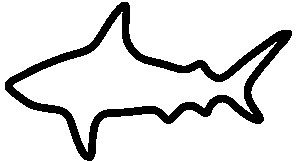
\includegraphics[width=4.5cm]{./sharc_logo.png}};

%%%%%%%%%%%%

%%%% SchNetPack Module

\draw[fill=white!50!ocp, draw=none, rounded corners=4pt] (6.35,3.3) rectangle (9.05,6.6);

\node[font=\sansmath\sffamily\small, black, bag] at (7.7,6.40) {$\mathtt{SchNetPack~2.0}$};

\draw[draw=black!50!ocp, fill=white!10!ocp, line width=0.75pt] (6.5,6.1) rectangle node[font=\sansmath\sffamily\small, black, bag]{$\mathtt{spk.representation}$ \\[1pt] \scriptsize{$\mathsf{(SchNet, PaiNN)}$}} (8.9,5.35);

\draw[draw=black!50!ocp, fill=white!10!ocp, line width=0.75pt] (6.5,5.1) rectangle node[font=\sansmath\sffamily\small, black, bag]{$\mathtt{spk.NeuralNetwork}$ \\ $\mathtt{Potential}$} (8.9,4.3);

\draw[draw=black!50!ocp, fill=black!40!ocp, line width=0.75pt] (6.5,4.2-0.15) rectangle node[font=\sansmath\sffamily\small, white, bag]{$\mathbf{ML~model}$} (8.9,3.45);

\draw[black, line width=0.8pt, ->] (7.7,5.35) -- (7.7,5.1);
\draw[black, line width=0.8pt, ->] (7.7,4.3) -- (7.7,4.05);
%%%% Loss Module

\draw[black, line width=0.8pt, dotted, line cap=round] (8.9,5.1) -- (9.45,6.6);
\draw[black, line width=0.8pt, dotted, line cap=round] (8.9,4.3) -- (9.45,3.3);
\draw[fill=none, draw=black, line width=0.8pt, dotted, line cap=round] (9.45,3.3) rectangle (11.9,6.6);
\node[font=\sansmath\sffamily\small, black, rotate=90] at (9.25,4.8) {$\mathsf{output~modules}$};

\node[font=\sansmath\sffamily\small, black, anchor=west, bag] at (9.55,4.9) {$\mathtt{\textcolor{HH}{spainn.loss.}}$ \\ $\mathtt{\textcolor{HH}{PhaseLoss}}$ \\ \scriptsize{$\mathsf{and}$} \\ $\mathtt{\textcolor{HH}{PhysPhaseLoss}}$ \\ \scriptsize{$\mathsf{(bulk~properties,}~ \mathbf{\mu}_{ji})$} \\[5pt] \textcolor{HH}{$\mathtt{PhaseLoss}$-} \\ \scriptsize{$\mathsf{and}$} \\ \textcolor{HH}{$\mathtt{PhysPhaseLoss}$-} \\ \textcolor{HH}{$\mathtt{Atomwise}$} \\ \scriptsize{$\mathsf{(atomistic~properties,}~ \mathbf{C}_{ji})$}};

%%%%% Prediction Modules

\draw[black, line width=0.8pt, dotted, line cap=round] (6.5,5.1) -- (5.85,5.2);
\draw[black, line width=0.8pt, dotted, line cap=round] (6.5,4.3) -- (5.85,0.5);
\draw[fill=none, draw=black, line width=0.8pt, dotted, line cap=round] (3.20,0.5) rectangle (5.85,5.2);

\node[font=\sansmath\sffamily\small, black, rotate=90] at (6.05,4.0) {$\mathsf{prediction~modules}$};

\draw[draw=black!30!gray, fill=white, rounded corners=5pt, line width=1pt] (3.3,5.1) rectangle node[font=\sansmath\sffamily\small, black, bag]{$\mathtt{\textcolor{HH}{spainn.Atomwise}}$ \\[1pt] \scriptsize{$\mathsf{atomistic~invariant~properties}$} \\ \scriptsize{$\mathsf{(\mathit{e.g.},~energies}~E_j)$}} (5.75,4.00);

\draw[draw=black!30!gray, fill=white, rounded corners=5pt, line width=1pt] (3.3,3.9) rectangle node[font=\sansmath\sffamily\small, black, bag]{$\mathtt{\textcolor{HH}{spainn.Forces}}$  \\[1pt] \scriptsize{$\mathsf{first~derivative~of~energy~per}$} \\ \scriptsize{$\mathsf{state~per~atom}~(-\nabla_{\mathbf{R}}E_j)$}} (5.75,2.85);

\draw[draw=black!30!HH, fill=white!98!HH, rounded corners=5pt, line width=1pt] (3.3,2.75) rectangle node[font=\sansmath\sffamily\small, black, bag]{$\mathtt{\textcolor{HH}{spainn.Nacs}}$ \\[1pt] \scriptsize{$\mathsf{nonadiabatic~couplings~be\text{-}}$} \\[-1pt] \scriptsize{$\mathsf{tween~electronic~states}~(\mathbf{C}_{ji})$}} (5.75,1.7);

\draw[draw=black!30!HH, fill=white!98!HH, rounded corners=5pt, line width=1pt] (3.3,1.6) rectangle node[font=\sansmath\sffamily\small, black, bag, yshift=-0.15mm]{$\mathtt{\textcolor{HH}{spainn.Dipoles}}$ \\[0.5pt] \scriptsize{$\mathsf{permanent~and~transition}$} \\[-1pt] \scriptsize{$\mathsf{dipole~moments}~(\mathbf{\mu}_{ji})$} } (5.75,0.6);

%%%% SPAINN

\node[font=\sansmath\sffamily\small, HH, bag] at (4.5,6.40) {$\mathtt{spainn.SPAINN}$};

\draw[draw=black!50!HH, fill=black!30!HH, rounded corners=4pt, line width=0.75pt] (3.3,6.1) rectangle node[font=\sansmath\sffamily\small, white, bag]{$\mathbf{datamodule}$ \\[1pt] \scriptsize{$\mathsf{(splitting, transform)}$}} (5.75,5.35);

\draw[black, line width=0.8pt, ->] (5.75,5.7) to node[above, black, font=\sansmath\sffamily\small, xshift=-0.5mm]{$\mathbf{R}, Z$} (6.5,5.7);

%\node[font=\sansmath\sffamily\small, HH, bag] at (4.5,6.40) {$\mathtt{spainn.SPAINN}$};

%%%% asetools

\node[font=\sansmath\sffamily\small, HH, bag] at (1.9,6.40) {$\mathtt{spainn.asetools}$};

\draw[draw=black!60!HH, fill=black!50!HH, rounded corners=4pt, line width=0.8pt] (0.1,6.15) rectangle node[font=\sansmath\sffamily\small, white, rotate=90]{$\mathtt{GenerateDB}$} (0.55,2.3);

\draw[draw=white!40!HH, fill=white!30!HH, rounded corners=4pt, line width=0.8pt] (0.1,2.2) rectangle node[font=\sansmath\sffamily\small, black, rotate=90]{$\mathtt{ConvertDB}$} (0.55,0.45);

%%%
\draw[draw=black!60!HH, fill=black!50!HH, rounded corners=4pt, line width=0.8pt] (0.9,6.1) rectangle node[font=\sansmath\sffamily\small, white, bag]{$\mathbf{parse~QM~data}$ \\ \scriptsize{$\mathsf{(SHARC/Molcas,\ldots)}$}} (2.9,5.4);

\draw[draw=black!60!HH, fill=black!50!HH, rounded corners=4pt, line width=0.8pt] (0.9,5.15) rectangle node[font=\sansmath\sffamily\small, white, bag]{$\mathbf{QM~properties}$ \\[1pt] \scriptsize{$\mathbf{R}, Z, E_j, \mathbf{F}_{j}, \textcolor{white!60!HH}{\mathbf{C}_{ji}}$}} (2.9,4.35);

\draw[draw=black!60!HH, fill=black!50!HH, rounded corners=4pt, line width=0.8pt] (0.9,4.1) rectangle node[font=\sansmath\sffamily\small, white, bag]{$\mathbf{transform~NACs}$ \\[1pt] \scriptsize{$\textcolor{white!60!HH}{\mathbf{C}_{ji}^{s}} = (\Delta{}E_{ji})^{-1}\textcolor{white!60!HH}{\mathbf{C}_{ji}}$}} (2.9,3.35);

\draw[draw=black, fill=black!50!HH, rounded corners=4pt, line width=0.75pt] (0.9,3.1) rectangle node[font=\sansmath\sffamily\small, white, bag]{$\mathtt{SPaiNN}~\mathbf{DB}$ \\[1pt] \scriptsize{$\mathbf{R}, Z, E_j, \mathbf{F}_{j}, \textcolor{white!60!HH}{\mathbf{C}_{ji}}, \textcolor{white!60!HH}{\mathbf{C}_{ji}^s}$}} (2.9,2.35);

\draw[draw=white!40!HH, fill=white!30!HH, rounded corners=4pt, line width=0.8pt] (0.9,2.10) rectangle node[font=\sansmath\sffamily\small, black, bag]{$\mathbf{convert~data}$ \\ \scriptsize{$\mathsf{(reshape~properties)}$}} (2.9,1.45);

\draw[draw=white!40!HH, fill=white!30!HH, rounded corners=4pt, line width=0.8pt] (0.9,1.2) rectangle node[font=\sansmath\sffamily\small, black, bag]{$\mathtt{SchNarc}~\mathbf{DB}$ \\ \scriptsize{$\mathbf{R}, Z, E_j, \mathbf{F}_{j}, \textcolor{black!30!HH}{\mathbf{C}_{ji}}$}} (2.9,0.5);

\draw[black, line width=0.8pt,smooth, ->, rounded corners] (2.9,2.70) to (3.05,2.7) to (3.05,5.75) to (3.3,5.75);
\draw[black, line width=0.8pt,smooth, ->, rounded corners] (0.9,1.80) to (0.7,1.8) to (0.7,3.7) to (0.9,3.7);

\draw[black, line width=0.8pt, ->] (1.9,5.4) -- (1.9,5.15);
\draw[black, line width=0.8pt, ->] (1.9,4.35) -- (1.9,4.1);
\draw[black, line width=0.8pt, ->] (1.9,3.35) -- (1.9,3.1);
\draw[black, line width=0.8pt, ->] (1.9,1.20) -- (1.9,1.45);

%%%%% SHARC

\draw[fill=black!60!white, draw=none, rounded corners=1pt] (6.9,2.9) rectangle (11.7,2.4);
\node[anchor=west, font=\sansmath\sffamily\scriptsize, white] at (10.9,2.65) {$t$};

\node[anchor=west, font=\sansmath\sffamily\scriptsize, fill=black!30!white, draw=none, rounded corners=1pt] at (8.0-1.0,2.65) {$\mathsf{\vphantom{\nabla_{R}}}\mathbf{R}, Z$};
\node[anchor=west, font=\sansmath\sffamily\scriptsize, fill=white!30!sii, draw=none, rounded corners=1pt] at (8.97-1.0,2.65) {$\nabla_R E_j$};
\node[anchor=west, font=\sansmath\sffamily\scriptsize, fill=white!30!sii, draw=none, rounded corners=1pt] at (9.85-1.0,2.65) {$\vphantom{\mathsf{\mathbf{\nabla_{R}}}E_j}C_{ji}, H_{ji}$};
\node[anchor=west, font=\sansmath\sffamily\scriptsize, fill=white!30!sii, draw=none, rounded corners=1pt] at (10.82-1.0,2.65) {$\vphantom{\mathsf{\mathbf{\nabla_{R}}}E_j}c_j$};
\node[anchor=west, font=\sansmath\sffamily\scriptsize, fill=white!30!sii, draw=none, rounded corners=1pt] at (11.32-1.0,2.65) {$\vphantom{\mathsf{\mathbf{\nabla_{R}}}E_j}\mathsf{j}$};

\draw[fill=black!30!white, draw=none, rounded corners=1pt] (6.9,1.6) rectangle (11.7,1.1);
\node[anchor=west, font=\sansmath\sffamily\scriptsize, white] at (10.9,1.35) {$t + \Delta{}t$};

\node[anchor=west, font=\sansmath\sffamily\scriptsize, fill=black!70!white, draw=none, rounded corners=1pt] at (8.0-1.0,1.35) {\textcolor{white}{$\mathsf{\vphantom{\nabla_{R}}}\mathbf{R}, Z$}};
\node[anchor=west, font=\sansmath\sffamily\scriptsize, fill=black!50!sii, draw=none, rounded corners=1pt] at (8.97-1.0,1.35) {\textcolor{white}{$\nabla_R E_j$}};
\node[anchor=west, font=\sansmath\sffamily\scriptsize, fill=black!50!sii, draw=none, rounded corners=1pt] at (9.85-1.0,1.35) {\textcolor{white}{$\vphantom{\mathsf{\mathbf{\nabla_{R}}}E_j}C_{ji}, H_{ji}$}};
\node[anchor=west, font=\sansmath\sffamily\scriptsize, fill=black!50!sii, draw=none, rounded corners=1pt] at (10.82-1.0,1.35) {\textcolor{white}{$\vphantom{\mathsf{\mathbf{\nabla_{R}}}E_j}c_j$}};
\node[anchor=west, font=\sansmath\sffamily\scriptsize, fill=black!50!sii, draw=none, rounded corners=1pt] at (11.32-1.0,1.35) {\textcolor{white}{$\vphantom{\mathsf{\mathbf{\nabla_{R}}}E_j}\mathsf{j}$}};

%%% step 1

\draw[HH, line width=1pt, rounded corners, smooth, line cap=round, ->] (7.3,2.85) to node[font=\sansmath\sffamily\scriptsize, left, yshift=-0.5mm]{\circled{$\mathsf{1}$}} (7.3,3.45);
\draw[HH, line width=1pt, rounded corners, smooth, line cap=round, ->] (7.5,3.45) to (7.5,3.10) to (8.35,3.10) to (8.35,2.85);
\draw[HH, line width=1pt, rounded corners, smooth, line cap=round, ->] (7.5,3.45) to (7.5,3.10) to (9.25,3.10) to (9.25,2.85);

%%% step 2

\draw[black!30!gray, line width=0.8pt, rounded corners, smooth, line cap=round, ->] (7.3,2.45) to (7.3,1.55);
\draw[black!30!gray, line width=0.8pt, rounded corners, smooth, line cap=round, ->] (8.35,2.45) to (8.35,2.15) to node[font=\sansmath\sffamily\scriptsize, below, yshift=-0.05mm]{\circled{$\mathsf{2}$}}  (7.3,2.15) to (7.3,1.55);

%%% step 3

\draw[HH, line width=1pt, rounded corners, smooth, line cap=round, ->] (7.25,1.15) to (7.25,1.00) to (6.8,1.00) to (6.8,3.45);
\draw[HH, line width=1pt, rounded corners, smooth, line cap=round, ->] (6.65,3.45) to node[font=\sansmath\sffamily\scriptsize, left, yshift=-5.05mm]{\circled{$\mathsf{3}$}} (6.65,0.90) to (8.20,0.90) to (8.20,1.15);
\draw[HH, line width=1pt, rounded corners, smooth, line cap=round, ->] (6.65,3.45) to (6.65,0.90) to (9.25,0.90) to (9.25,1.15);


%%% step 4

\draw[black!30!gray, line width=0.8pt, rounded corners, smooth, line cap=round, ->] (9.95,2.45) to (9.95,1.55);
\draw[black!30!gray, line width=0.8pt, rounded corners, smooth, line cap=round, ->] (9.25,2.45) to (9.25,2.15) to (9.95,2.15) to (9.95, 1.55);
\draw[black!30!gray, line width=0.8pt, rounded corners, smooth, line cap=round, ->] (9.25,1.55) to (9.25,2.15) to node[font=\sansmath\sffamily\scriptsize, below, yshift=-0.05mm]{\circled{$\mathsf{4}$}} (9.95,2.15) to (9.95, 1.55);

%%% step 5

\node[anchor=west, font=\sansmath\sffamily\scriptsize, fill=black!50!theo, draw=none, rounded corners=1pt] at (10.7,2.1) {\textcolor{white}{$h$}};

\draw[black!30!gray, line width=0.8pt, rounded corners, smooth, line cap=round, ->] (10.05,2.45) to (10.05,2.15) to (10.7, 2.15);
\draw[black!30!gray, line width=0.8pt, rounded corners, smooth, line cap=round, ->] (10.45,2.45) to (10.45,2.15) to (10.7, 2.15);
\draw[black!30!gray, line width=0.8pt, rounded corners, smooth, line cap=round, ->] (10.7,2.05) to (10.45,2.05) to node[font=\sansmath\sffamily\scriptsize, left, yshift=1.1mm]{\circled{$\mathsf{5}$}} (10.45, 1.55);

%%% step 6

\draw[black!30!gray, line width=0.8pt, rounded corners, smooth, line cap=round, ->] (10.45,1.15) to (10.45,0.70) to node[font=\sansmath\sffamily\scriptsize, above, xshift=5mm, yshift=-0.3mm]{\circled{$\mathsf{6}$}} (8.45, 0.7) to (8.45,1.15);
\draw[black!30!gray, line width=0.8pt, rounded corners, smooth, line cap=round, ->] (7.35,1.15) to (7.35,0.70) to (8.45,0.70) to (8.45,1.15);

%%%%%%%%%5

\node[font=\sansmath\sffamily\small, HH, anchor=west, bag] at (6.10,0.45) {\texttt{spainn.calculator.SPaiNNulator}};

\node[font=\sansmath\sffamily\small, black!30!gray, anchor=west, bag] at (10.45,0.76) {\texttt{SHARC~3.0}};


\end{tikzpicture} 
\end{document}

